%% ==============================================
%%           Design and Implementation
%% ==============================================
%% Author: Fabian Sorn
%% ==============================================


\chapter{Design and Implementation of a Benchmark Framework}
\label{ch:application}

In this chapter, the findings from the previous chapters will be combined to
design and implement a benchmarking framework, which allows users to
benchmark specific charting operations. 


%% ==============================================
%%          Python Graph Libraries
%% ==============================================

\section{Python Graph Libraries} \label{sec:application:libraries}

When benchmarking different Python Graph libraries, we will focus our attention
on two popular contenders for the implementation, which are very well accepted
in the scientific community.

\subsection{Matplotlib} \label{sec:application:libraries:matplotlib}

Matplotlib is without a doubt the standard library for 2D data visualization in
Python. It offers publication quality visualization as well as an interactive
environment. The project was initialized by John D. Hunter as an easy to use
Python 2D plotting library, especially for users familiar with Data
Visualization in Matlab.
\cite{Matplotlib, MatplotlibHistory}

Matplotlib's central item is the \inlinecode{Python}{matplotlib.figure.Figure}.
The Figure itself does not yet display anything, neither a plot with axes nor
data. A plot is referred as an \inlinecode{Python}{matplotlib.axes.Axes}. A
figure can have multiple Axes in it. For each dimension in the data space the
Axes contains \inlinecode{Python}{matplotlib.axis.Axis} objects, which
represents the minimum and maximum data limit for each dimension of the data. An
Axes object can be personalized through axis labels and a title. In Matplotlib
terminology, Artists are everything which is visible in a Figure. This includes
Labels, Lines and Bar Graphs, Axis Items and more. The last crucial component is
the Canvas, which is not really a visual component in the plot, but the
component responsible for rendering the image. A summary of all components can
be seen in \ref{a:fig:matplotlib:content}

Matplotlib is built for many different use cases. While showing data in
\gls{gui} applications is one of them, other use cases, like generating plots as
images for publications are possible as well. This is achieved by Matplotlib's
different backends. All available Backends can be divided in interactive and
hard copy ones. An example for a interactive backend is in our case PyQt5, but
other Frameworks like Tkinter or PyGTK are supported as well. Non interactive
backends are for creating image files in different file formats like PNG, SVG,
PDF and more.
\cite{MatplotlibIntro, PythonDataVis}

Listing \ref{listing:application:matplotlib} shows the creation of a window
containing a plot representing a sinus curve through a line, a scatter plot and
a bar graph. For interaction, matplotlib offers a toolbar, which lets you select
between different interaction modes like panning and zooming. As a backend
Matplotlib's Qt5 backend was used.  The resulting window can be seen in
Screenshot \ref{a:fig:matplotlib:window}.

\lstinputlisting[ 
    caption=Definition of a Window containing a plot created with Matplotlib,
    language=python,
    label=listing:application:matplotlib,
    firstline=4,
    lastline=32
]{resources/code/matplotlib_demo.py}

\subsection{PyQtGraph} \label{sec:application:libraries:pyqtgraph}

PyQtGraph is a pure python plotting library. Even though it does not offer as
many features as other Python plotting libraries like Matplotlib, PyQtGraph
promises much better performance. The project was initialized by Luke Campagnola
and is focused on providing plotting functionalities for engineering and science
applications. It provides simple plots containing line graphs, scatter plots,
bar graphs and more, but also image and video displaying, Region of Interest
widgets, 3D visualization and more.  Since our benchmarking efforts will be
tightly focusing on the collected use cases, we will restrict our usage of its
features mainly on two dimensional plotting. PyQtGraph uses Qt's Graphics View
for drawing, which is a Framework for fast visualization of a large number of
custom 2D items. A big advantage it offers is a fast performance and the
possibility to interact and transform the scene through operations like
zooming or rotation.
\cite{GraphicsView}

Since PyQtGraph is built on top of Qt features, integrating it into Qt
applications is very simple. The central component for plotting is the
\inlinecode{Python}{pyqtgraph.PlotWidget}, which is derived from
\inlinecode{Python}{QtWidgets.QWidget}. When adding the plot widget to a
window, it comes with different components on the inside, as seen in
\ref{a:fig:pyqtgraph:content}. The central one is the
\inlinecode{Python}{pyqtgraph.PlotItem}, which is the actual plot. The widget
itself is only a wrapper for easy integration into Qt Applications. The plot
item contains different components of the plot, including a
\inlinecode{Python}{pyqtgraph.ViewBox}, the area data is visualized in,
a \inlinecode{Python}{pyqtgraph.AxisItem} representing the View Range
of the View Box, and a Title. Items which are actually representing a dataset are
added to the View Box. For this, PyQtGraph is offering different types of
representations like \inlinecode{Python}{pyqtgraph.PlotDataItem} for Scatter
Plots and Line Graphs and \inlinecode{Python}{pyqtgraph.BarGraphItem} for
representing data in a bar graphs.

Listing \ref{listing:application:pyqtgraph} shows the creation of a window
containing a plot representing a sinus curve in different ways. It displays the
same data sets in the same style as the Matplotlib example
\ref{sec:application:libraries:matplotlib}. The resulting window can be seen in
\ref{a:fig:pyqtgraph:window}.
\cite{PyQtGraphDoc}

\lstinputlisting[
    caption=Definition of a window containing a plot created with PyQtGraph,
    language=python,
    label=listing:application:pyqtgraph,
    firstline=2,
    lastline=25
]{resources/code/pyqtgraph_demo.py}


%% ==============================================
%%                   Analysis
%% ==============================================

\section{Analysis}
\label{sec:application:analysis}

After having a closer look at the two plotting libraries, this chapter will
focus on the analysis of the requirements which we will base the design and
implementation of our framework on.

Users interested in the performance of graph libraries often have a very clear
idea of what their use case looks like, since they already know the background
information of the data they want to plot. Because of this, the central
interface to the framework should be these use cases. Most higher level use
cases can be broken down in a simple operation or a sequence of operations. From
our collected use cases we can define the following requirements.

\begin{description}
    \item[Ease of Use] 
        The user should only define the relevant parts for his use cases.
        Everything else should be handled by the framework.
    \item[Widget and Operation]
        The central items for defining a use case are a widget, and an operation
        which is executed on this widget.
    \item[Multiple Use Cases]
        Adding and removing use cases has to be possible without much effort.
    \item[Parameterization]
        A use case has to be reusable for different parameters and has to be
        easily extensible.
    \item[Performance Expectations]
        The author has to be able to define his performance expectations per use
        case.
    \item[Timeout]
        In case a use case takes much longer than expect, it should be possible
        to define a timeout, which will terminate the use case's execution, if
        reached.
\end{description}

One framework type, which allows a very similar way of defining specific use
cases, are testing frameworks like unittest or pytest for python projects. Since
most users are to an extend familiar with their functionality, the interface
should conform the expectations built from the usage of these frameworks.

For easy execution of use cases, the framework will offer a command line
interface, which offers similar functionality as other python tools. The
\gls{cli} should conform the user's expectations in the same way with a few
additions specific to our needs. 

\begin{description}
    \item[Use Case Exection]
        Similar to frameworks like pytest, it should be able to execute multiple
        use cases as well as single ones.
    \item[Meaningful Results]
        After execution, the user should be able to clearly see the results of
        his use cases. This includes the use case, its performance requirements,
        the actually achieved performance and the parameters used in the run.
    \item[Profiling]
        Since Profiling introduces additional overhead to the code's execution,
        profiling should be optional and activatable through the \gls{cli}.
    \item[Profiling Visualization]
        Since profiles often contain large amount of data, they have to be
        visualized in a user friendly way.
\end{description}


%% ==============================================
%%                  Design
%% ==============================================

\section{Design}

\label{sec:application:design}

This section will focus on describing the design of the framework. The most
outer layer contains two components: the command line interface and the business
logic. The command line interface offers the user the possibility to start the
execution of his benchmarking use cases. Additionally it is responsible for
presenting the results after the execution finished. The second component is the
business logic, which is responsible for providing interfaces for defining use
cases, the logic for executing them, as well the functionality to record the
achieved results. We will refer to the executing part of the framework as the
launcher from now on.

\subsection{Benchmark Execution}

Figure \ref{fig:application:design:cli} shows the communication between the
user, the command line interface and the launcher when executing use cases from
the command line.  When the user starts the framework's executable, a \gls{cli}
instance is created, which parses the command line arguments and instantiates
the launcher. To keep the user interface exchangeable, launcher and \gls{cli}
are strictly separated from each other. The launcher will import the passed use
case modules, with which the initialization is completed. To start the
execution, the launcher offers a \inlinecode{Python}{run()} method. Each
collected use case will then be executed sequentially and its achieved results
collected. After all use cases are executed and all results are available, they
are passed back the \gls{cli}, where they can be presented to the user.

\begin{figure}[h]
    \centering
    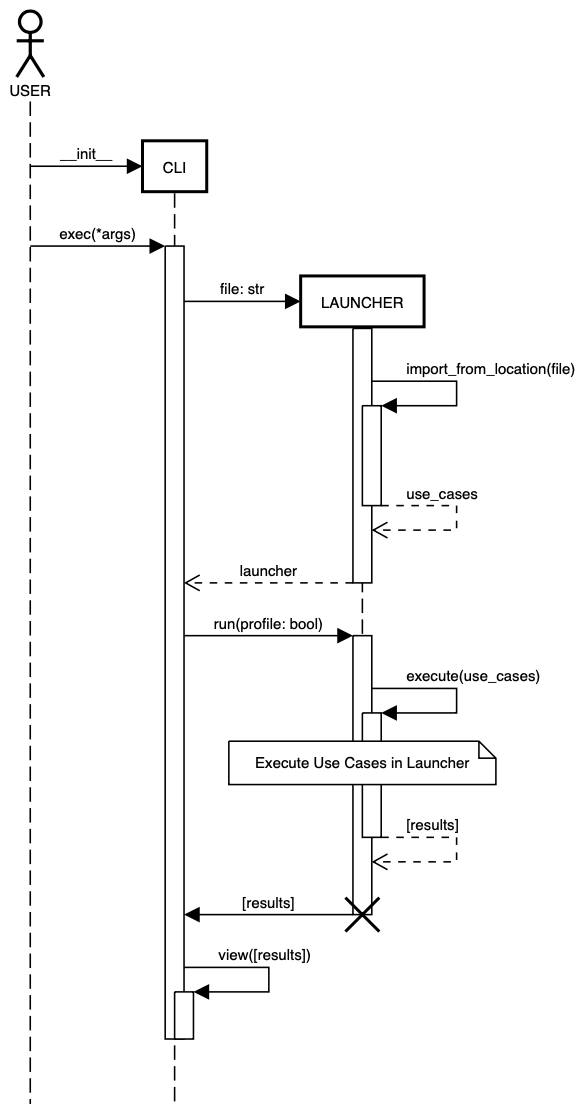
\includegraphics[width=11cm]{resources/img/sequence/cli}
    \caption{
        Sequence diagram showing the communication between the command line
        interface and the business logic.
    }
    \label{fig:application:design:cli}
\end{figure}


Next we will have a more detailed look at the inner workings of the launcher.
Its central task is the execution of use cases, which is visualized in depiction
\ref{fig:application:design:launcher}. Our goal is to allow executing a suite of
use cases similar to testing frameworks allowing the execution of entire test
suites at once. Each use case will have to be executed sequentially and in a
separate environment, to prevent different use cases having an influence on each
other.  The same principle applies to parameterized use cases. This means the
execution will take place in a nested loop with the outer one cycling through
the use cases and the inner one through its parameter combinations.

Visualization \ref{fig:application:design:launcher} introduces two new
components, which build the execution environment for a single use case. The
first component is the window, which will house our widget, on which we want to
operate. The second component is the executor, which is responsible for
executing the defined operation on the window and record timing information and
profiling statistics. After our Launcher is initialized and our benchmark files
are fully imported, we will execute each use case in all possible parameter
combinations. For each combination we create a new benchmarking window. The
window will then be passed to the executor. The executor will access all use
case related information and operations through this window reference. For
starting the execution, the executor offers a \inlinecode{Python}{run()}
function, which gets called by the launcher.

\begin{figure}[h]
    \centering
    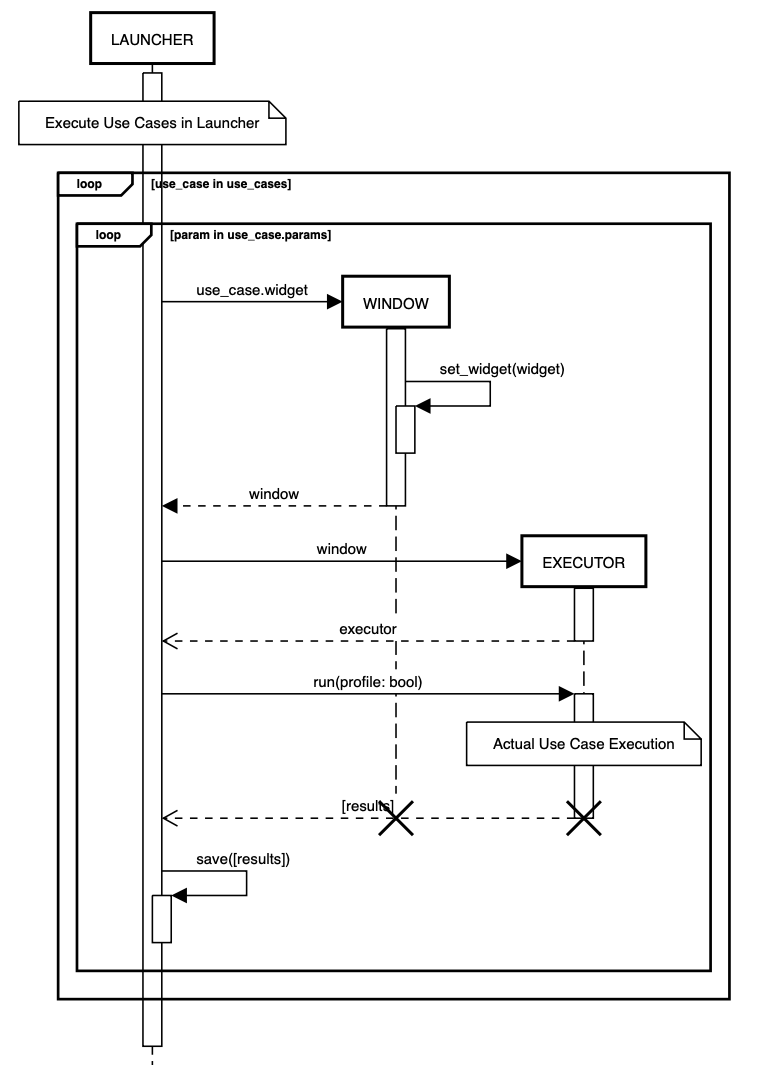
\includegraphics[width=12cm]{resources/img/sequence/launcher}
    \caption{
        Sequence diagram showing the execution of a set of use cases in more
        detail.
    }
    \label{fig:application:design:launcher}
\end{figure}

Depiction \ref{fig:application:design:executor} shows the execution of a single
use case in more detail. Before each operation, the current time stamp is taken.
If a profile is supposed to be created, the profiler is started right after
that.  Next the operation, which we want to benchmark, is executed on the passed
window reference. After it and all of its side effects are completed, the
profiler is stopped if necessary. Its statistics are added to the already
collected ones. This execution cycle is repeated, until the defined repeat count
or the timeout is reached. At the end, the timing information and the profiling
statistics will be returned to the launcher.

\begin{figure}[h]
    \centering
    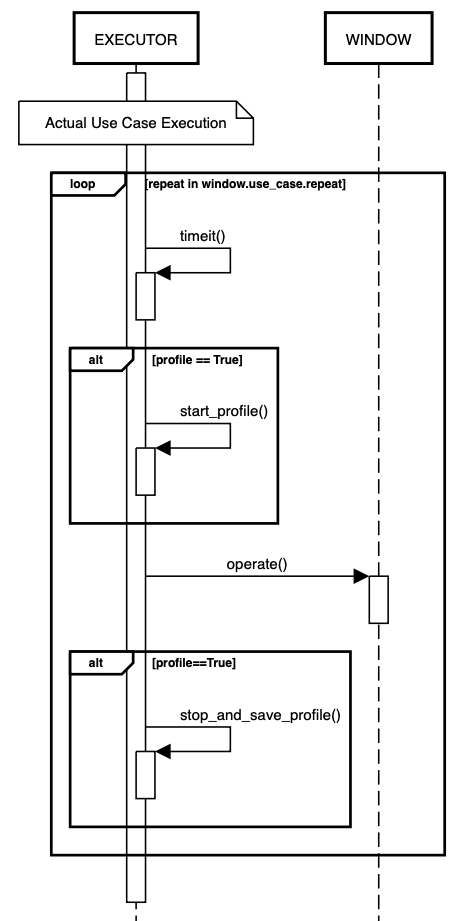
\includegraphics[width=8cm]{resources/img/sequence/executor}
    \caption{
        Sequence diagram showing the actual benchmarking execution on the window
        by the executor in more detail.
    }
    \label{fig:application:design:executor}
\end{figure}

Figure \ref{fig:application:design:classdiagram:widgetmark} shows a class
diagram of all classes involved in the sequence diagrams and their relationships
to each other. Additionally it shows the use case interface with all its
attributes and functions based on our analysis in section
\ref{sec:application:analysis}. To define a new use case, the user can subclass
this class and implement all necessary components. The results of a single use
case are represented by its own class, which can be passed between each of the
components involved in the execution until they can be display by the \gls{cli}.

\begin{figure}[h]
    \centering
    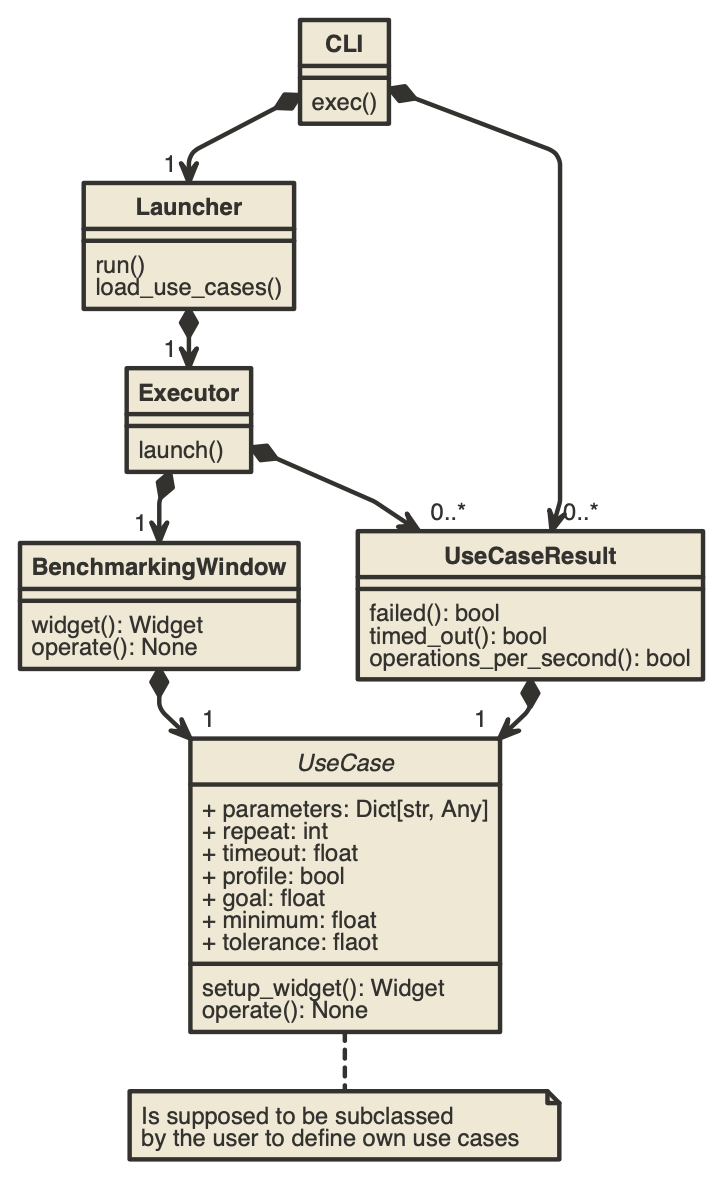
\includegraphics[width=8cm]{resources/img/class/widgetmark}
    \caption{
        Class diagram depicting all important classes involved in the
        Benchmarking Framework. 
    }
    \label{fig:application:design:classdiagram:widgetmark}
\end{figure}

\clearpage

\subsection{Use Case Definition and Plotting Abstraction Layer}

\label{sec:application:design:usecases}

In this section we will have a closer look at definition of use cases based on
the requirements collected in section \ref{sec:application:analysis}. A
single use case is represented by a class implementing the
\inlinecode{Python}{UseCase} interface. One python module can contain multiple
of these use case classes. By only executing classes derived from the use case
interface, we can allow defining other classes in the same modules as well
without them being executed by accident.

To define plotting benchmarks that are executable with different plotting
libraries we will define a unified interface for them. For the purpose of this
work, we will limit this interface to the functionality needed to execute our
use cases. In general this interface is limited to operations supported by all
graph libraries implementing it. With using the parameterization functionalities
of our use case interface, we can define higher level plotting benchmarks and
execute them using different libraries to compare the results from each of them.

\begin{figure}[h]
    \centering
    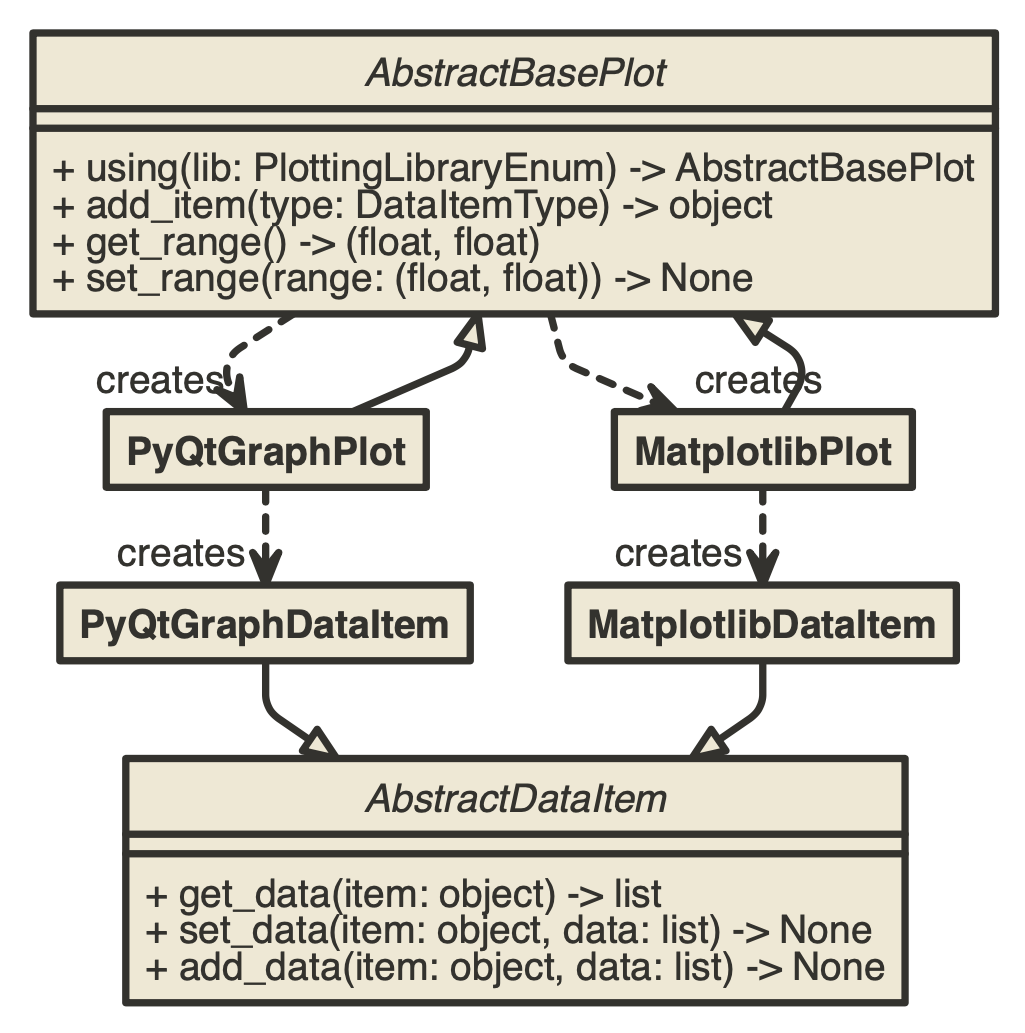
\includegraphics[width=7cm]{resources/img/class/plotabstraction}
    \caption{
        Class diagram depicting the plot abstraction interface and two
        subclasses for the python plotting libraries PyQtGraph and Matplotlib. 
    }
    \label{fig:application:design:classdiagram:plot}
\end{figure}

Figure \ref{fig:application:design:classdiagram:plot} shows the abstract base
classes for the plot widget as well as data items like curves, bar graphs,
scatter plots and more. The class \inlinecode{Python}{AbstractBasePlot} offers
plot functionalities to add a new item, get and set the current view range and a
factory method for creating a plot using a specific plotting library. The two
subclasses \inlinecode{Python}{PyQtGraphPlot} and
\inlinecode{Python}{MatplotlibPlot} can implement the functionality defined by
the base class using their specific \gls{api}. The
\inlinecode{Python}{AbstractDataItem} on the other hand defines a common
interface for setting, getting and adding new data to a data item of a plot.
Similar to the \inlinecode{Python}{AbstractBasePlot}, this interface is
implemented by the two subclasses \inlinecode{Python}{PyQtGraphDataItem} and
\inlinecode{Python}{MatplotlibDataItem} using their specific \gls{api}.

Listing \ref{listing:application:plotabstraction} shows, how the interface
should be usable in a standard Qt application. Which library is used for the
visualization can be controlled during the widget's initialization using the
\inlinecode{Python}{AbstractBasePlot} factory method
\inlinecode{Python}{using()}.

\lstinputlisting[ 
    caption=Creating a plot showing a sinus curve using the Plot Abtraction 
            Layer,
    language=python,
    label=listing:application:plotabstraction,
    firstline=9,
    lastline=30
]{resources/code/plot_abstraction.py}


\subsection{User Interface}

In this section we will have a look at the design of the command line interface
based on the requirements we collected in \ref{sec:application:analysis}. Since
our command line is supposed to be easily usable for users of other testing
frameworks, it should meet the user's expectations. The main purpose of the
command line is starting the execution of one or multiple use cases. Listing
\ref{listing:application:cliusage:location} shows how to specify, which use
cases should be executed. It should be possible to define a folder, a python
module or a specific use case inside a python module. For python modules
containing use cases, we will introduce a specific naming convention. The
default one should be, that the python module's name is prefixed with
\inlinecode{bash}{bench_}, similar to test files being often prefixed with
\inlinecode{Python}{test_}. This pattern should be configurable from the
command line as well.

\lstinputlisting[ 
    caption=Executing use cases from the command line,
    language=bash,
    label=listing:application:cliusage:location,
    lastline=39
]{resources/code/widgetmark_cli_usage.sh}

Additionally the command line should allow us to configure, if we want to run
the framework with or without profiling, as well as the location the files are
saved in. Listing \ref{listing:application:cliusage:profile} shows these
configuration options on the command line as well as the generated files.

\lstinputlisting[ 
    caption=Starting benchmarks and create profiles for them,
    language=bash,
    label=listing:application:cliusage:profile,
    firstline=40,
    lastline=52
]{resources/code/widgetmark_cli_usage.sh}

Additionally the \gls{cli} should provide a visualization option for the
profiling statistics. Simply printing the profiling statistics to the command
line would not be very helpful, since they can grow very fast in size. Because
of this, there are multiple tools available, which offer a much more user
friendly visualization. For our purposes we decide for \emph{snakeviz}, a
browser based graphical viewer for profiling files.  \cite{Snakeviz}

To improve the usability of the \gls{cli}, a help function should be offered
which explains what the framework is and how it is going to be used.
Listing \ref{listing:application:cliusage:help} shows how such a help message
could look like. Additionally it should be possible to run the \gls{cli} with
additional output when searching for bugs in a use cases definition. 

\lstinputlisting[ 
    caption=Starting benchmarks and create profiles for them,
    language=bash,
    label=listing:application:cliusage:help,
    firstline=58,
    lastline=68
]{resources/code/widgetmark_cli_usage.sh}

After the execution is completed, the \gls{cli} output should show all
important information about the found files, the use cases, the performance
requirements, the parameters and the actual reached frame rate. Listing
\ref{listing:application:cliusage:output} shows, how these informations could be
presented.

\lstinputlisting[ 
    caption=Output of the CLI with showing the benchmark results,
    language=bash,
    label=listing:application:cliusage:output,
    firstline=69,
]{resources/code/widgetmark_cli_usage.sh}


%% ==============================================
%%             Implementation
%% ==============================================

\section{Implementation} \label{sec:application:implementation}

This section will focus on the actual implementation of the framework based on
the Analysis from section \ref{sec:application:analysis}, the design from
section \ref{sec:application:design} and the Use Cases from chapter
\ref{ch:usecases}. As a name we choose \emph{widgetmark}, a composite of widget
and benchmark.  The language we use is Python in the version 3.6 to use newer
language features like typing hint, which will highly improve the usability of
the framework.

\subsection{Project Structure}

The first part of the implementation is setting up our project in Python, which
figure \ref{fig:application:implementation:structure} is showing. The project
will follow python best practices with a package \emph{widgetmark} for the
source code and \emph{tests} for unit tests. Additionally the project contains
the two generated files \emph{\_version.py} and \emph{versioneer.py} for getting
version information from version control tags, \emph{README.md} for a
introduction into the project, \emph{setup.cfg} for tooling configuration and
\emph{setup.py} for dependency definition and installation instructions.

\begin{figure}[h]
    \centering
    \framebox[\textwidth]{%
        \begin{minipage}{0.9\textwidth}
            \dirtree{%
                .1 project.
                .2 widgetmark.
                    .3 base.
                        .4 benchmark.py.
                        .4 executor.py.
                        .4 launcher.py.
                    .3 qt.
                        .4 benchmark.py.
                        .4 executor.py.
                        .4 plot.py.
                        .4 util.py.
                    .3 cli.
                        .4 \_\_main\_\_.py.
                        .4 cli.py.
                        .4 cli\_view.py.
                        .4 loader.py.
                    .3 \_version.py.
                .2 tests.
                    .3 \_\_init\_\_.py.
                    .3 \dots.
                .2 setup.py.
                .2 setup.cfg.
                .2 versioneer.py.
                .2 README.md.
            }
        \end{minipage}
    }
    \caption{Widgetmark project structure}
    \label{fig:application:implementation:structure}
\end{figure}

\subsection{Subpackage widgetmark.base}

The first sub-package of our implementation is the package
\inlinecode{Python}{widgetmark.base}. In this package we will define all base
classes for our benchmarking framework, which are not part of the user
interface. To keep the framework extensible and not limited to Qt as its
\gls{gui} framework, we will skip qt specific implementations of functionality
in this package and only offer common functionality not related to \gls{gui}
operations. Qt specific implementations will be part of the
\inlinecode{Python}{widgetmark.qt} package.

\subsubsection*{benchmark.py}

The first class for our implementation is the use case interface. Python does
not support interfaces, but offers abstract classes we can use to define our
interface by simply not provide any implementations for functions.

\lstinputlisting[ 
    language=Python,
    linerange={2-2, 14-14}
]{resources/widgetmark/base/benchmark.py}

When distinguish three different types of information that can be
defined in a use case: functions all subclasses have to implement, attributes
subclasses have to implement and attributes subclasses can implement.
Mandatory functions can be simply implemented as abstract methods using the
\inlinecode{Python}{abstractmethod} decorator provided by the
\inlinecode{Python}{abc} package.

\lstinputlisting[ 
    language=Python,
    linerange={116-117, 124-124}
]{resources/widgetmark/base/benchmark.py}

Non mandatory attributes can be easily implemented as class attributes.

\lstinputlisting[ 
    language=Python,
    linerange={30-30}
]{resources/widgetmark/base/benchmark.py}

For implementing mandatory attributes, \inlinecode{Python}{abc} does not offer
any standard decorators, but we can use \inlinecode{Python}{property} in
combination with the \inlinecode{Python}{abstractmethod} decorator to create
abstract properties for out class. While such an implementation does not
actually depict a mandatory attribute on a class level, the abstract property
can be implemented as a class attribute in subclasses.

\lstinputlisting[ 
    language=Python,
    linerange={56-58, 64-64}
]{resources/widgetmark/base/benchmark.py}

\lstinputlisting[ 
    language=Python,
    linerange={19-19, 22-22}
]{resources/widgetmark/bench_label.py}

With this implementation, there is no visual difference between defining
mandatory or optional attributes in use case classes, but we can enforce, that
all all mandatory attributes have been implemented. Both, class attributes and
abstract properties can also be accessed the same way after the class is
initialized using \inlinecode{Python}{instance.attribute}.

The next class defined in this module is the \inlinecode{Python}{UseCaseResult}
class, which is based on a single use case. For parameterized use cases, there
will be a result instance for each parameter combination. The result object
should comprise all information we have recorded from the use case. To make sure
that use cases are read only after their initialization, we hold the information
in private instance attributes and allow reading access only over properties
without defining property setters. Additionally we offer convenient properties
for checks on the results. An example is a \inlinecode{Python}{failed} property
that can be used to check for exceptions instead of comparing the
\inlinecode{Python}{result.exception is None} property against
\inlinecode{Python}{result.failed}.

\lstinputlisting[ 
    language=Python,
    linerange={173-180, 194-198, 245-246, 248-248}
]{resources/widgetmark/base/benchmark.py}

The last class defined in the module is the benchmarking window, which
incorporates the widget defined in the use case and grants access to the
operation we want to benchmark. Wrapping the operation allows us to access it
later in the executor without having to keep a direct reference to the use case.
Since our goal is to keep the base implementation free from \gls{gui} framework
specific functionality, we won't subclass any Qt window classes like
\inlinecode{Python}{QtWidgets.QMainWindow}.

\subsubsection*{executor.py}

The executor module contains the class
\inlinecode{Python}{AbstractBaseExecutor}, which is responsible for executing
the benchmarking operations on the window, record the results and create a
fitting instance of the \inlinecode{Python}{UseCaseResult} class.

As \ref{fig:application:design:executor} shows, for recording execution times,
we need a loop like execution of the same operation over and over again. Simply
using a loop can lead to unrealistic results, since we have to give back the
control to the control loop in between operations to not skip on pending work
caused by our operation. The practical implementation of this is dependent on
the used \gls{gui} framework and will not be part of this class. As for the
benchmarking window, this implementation will be done in a fitting executor
subclass in package \inlinecode{Python}{widgetmark.qt}.

For all \gls{gui} independent functionalities, this class does provide
implementations. As seen in \ref{fig:application:design:executor} an executor
instance is initialized for every parameter combination of every use case. After
the initialization, a window can be attached to the executor through
\inlinecode{Python}{set_window()}. The execution can then be launched using the
\inlinecode{Python}{launch()} method. 

\lstinputlisting[
    language=Python,
    linerange={38-56}
]{resources/widgetmark/base/executor.py}

Internally the abstract protected function \inlinecode{Python}{_launch()} is
called, which gives \gls{gui} specific subclasses an opportunity to set up the
actual execution loop. This loop can use the protected operation
\inlinecode{Python}{_redraw_operation}, which is responsible for calling the
operation on the window, collect timing information and control the profiler.

\lstinputlisting[
    language=Python,
    linerange={107-121}
]{resources/widgetmark/base/executor.py}

For recording the current time-stamp we can use the \inlinecode{Python}{time()}
function of the python package \inlinecode{Python}{time}, which returns us the
current time as floating point number. From this time-stamp and the last
recorded one we can calculate the delta timing for the last step. The current
time will be saved in an instance attribute for the next operate.

\lstinputlisting[
    language=Python,
    linerange={154-159}
]{resources/widgetmark/base/executor.py}

The protected function \inlinecode{Python}{_profile} is responsible for
controlling the profiler, which is used to profile the use case operation and
combine the profiling stats from each step to a single profiling stat. Before
the old step the current Profile will be disabled, the stats are added to the
previously saved ones and the new profile will be enabled.

\lstinputlisting[
    language=Python,
    linerange={124-137}
]{resources/widgetmark/base/executor.py}

The last important function is \inlinecode{Python}{_check_if_completed()}
function, which stops execution if either the timeout or the repeat counter of
the use case is reached. If one is the case, the protected function
\inlinecode{Python}{_complete()} is called. Since reaching the end of the
execution cycle means stopping the execution loop, this step is \gls{gui}
framework specific and will be implemented in the subclasses. 

\lstinputlisting[
    language=Python,
    linerange={139-152}
]{resources/widgetmark/base/executor.py}

\subsubsection*{launcher.py}

The module \inlinecode{Python}{launcher} contains the class
\inlinecode{Python}{Launcher}. As figure \ref{fig:application:design:launcher}
shows, the purpose of the Launcher class is to create fitting benchmarking
windows and executors for the use cases it was passed on initialization. The
launcher can be initialized using either a list of types, which are derived from
the \inlinecode{Python}{UseCase} class or with a list of file locations, where
these classes are defined. If a list of files is passed, the fitting classes are
imported using the \inlinecode{Python}{importlib} module which python offers.
To make sure we import only classes that we want, we filter the found classes by
their name and their type. The filtering by name is for cases the user specifies
a specific name or name pattern on the command line, the type filtering is for
not accidentally trying to initialize classes which do not define use cases.
This way use case files can safely contain other class definitions without
leading to errors.

\lstinputlisting[
    language=Python,
    linerange={123-126, 133-154}
]{resources/widgetmark/base/launcher.py}

The initialized launcher instance can be started using the
\inlinecode{Python}{run()} method, which takes a parameter
\inlinecode{Python}{profile} for controlling if the executor will create a
profile of the use case or not. Before initializing window and executor we
create a list of all parameter combinations. For each of these parameter
combinations we initialize the use case class. To grant access in the use case
class to these parameters, we set them as instance attributes to the initialized
use case instance. If the use case class defines for example the parameters
\inlinecode{Python}{'number': [0, 1]}, we can access the value of this
parameter in the use case class during execution by calling 
\inlinecode{Python}{self.number}.

\lstinputlisting[
    language=Python,
    linerange={90-119}
]{resources/widgetmark/base/launcher.py}

To resolve the right window and executor implementation for the backend defined
by the use case, we have the class \inlinecode{Python}{BackendResolver} which
does iterates through a classes subclass using the underscore function
\inlinecode{Python}{__subclasses__()} to find one fitting to the requested
backend. For this each subclass defines a class attribute
\inlinecode{Python}{gui_backend}, which can be compared to the
\inlinecode{Python}{backend} class attribute of the use case classes.

\subsection{Subpackage widgetmark.qt}

This package contains qt specific implementations of the benchmarking window and
the executor, as well as the qt plotting interface.

\subsubsection*{benchmark.py}

This module provides a Qt based implementation of the
\inlinecode{Python}{AbstractBenchmarkingWindow} based on 
\inlinecode{Python}{QtWidgets.QMainWindow}. Since Python supports multi
inheritance, the Qt benchmarking window can be implemented as follows. The
\inlinecode{Python}{make_qt_abc_meta()} function in this class definition is for
solving the meta class conflict between qt classes and the
\inlinecode{Python}{ABCMeta} from the \inlinecode{Python}{abc} package. This is
achieved by returning a metaclass that is derived from both the meta class of
\inlinecode{Python}{QMainWindow} and \inlinecode{Python}{ABCMeta}. Its
implementation can be found in the \inlinecode{Python}{util.py} module of the
same package.

\lstinputlisting[
    language=Python,
    linerange={7-9}
]{resources/widgetmark/qt/benchmark.py}

\subsubsection*{executor.py}

This module provides a Qt based implementation of the
\inlinecode{Python}{AbstractBenchmarkExecutor} based on
\inlinecode{Python}{QtCore.QObject}. The executor has to start a Qt application
and implement two functions based on it: \inlinecode{Python}{_launch()} and
\inlinecode{Python}{_complete()}. Initialization of the benchmark execution loop is the
purpose of \inlinecode{Python}{_launch}. To make sure, that no pending events
are skipped, we want to give back control to Qt's event loop after each time our
operation we want to benchmark is executed. In Qt we can achieve such a loop
by using the \inlinecode{Python}{QtCore.QTimer} with a timeout of zero seconds.
Such a timer will timeout every time it is possible. 
\cite{QTimer}

To the timer's timeout signal we can connect the executor's base's
\inlinecode{Python}{_redraw_operation} function, which handles profiling, timing
and operation execution. After the timer is set up we can start the event loop
of our Qt application.

\lstinputlisting[
    language=Python,
    linerange={60-64}
]{resources/widgetmark/qt/executor.py}

After the executor's base notices in its
\inlinecode{Python}{_check_if_completed} function, that either the timeout or
the maximum repeat counter is reached, it will call the
\inlinecode{Python}{_complete} function. Its purpose is not only to wrap the
recorded performance figures in a \inlinecode{Python}{UseCaseResult} instance,
but also to stop the execution loop. Since the loop is based on a
\inlinecode{Python}{QtCore.QTimer}, we can use its \inlinecode{Python}{stop()}
function to achieve this.

\lstinputlisting[
    language=Python,
    linerange={66-77}
]{resources/widgetmark/qt/executor.py}

The Executor is also responsible to start and quit the
\inlinecode{Python}{QtWidgets.QApplication}. One caveat worth mentioning in this
context is, that there should only be a single instance of the application
running, since multiple \inlinecode{Python}{QApplication} instances will lead to
problems. Because of this, the executor class has to make sure, that there is
no existing one before creating a new one.

\lstinputlisting[
    language=Python,
    linerange={79-87}
]{resources/widgetmark/qt/executor.py}

Since the window and the widget is exposed during the benchmark execution, the
user is able to interact with it. Since these interactions are not part of the
use case, they would affect the results negatively, since their work effort
would be counted as work produced by the use case. Because of this, we have to
filter out all operations, which are not directly caused by operations of the
use case. As described in section \ref{sec:fundamentals:qt:eventloop}, Qt offers
us the possibility to install event filters, which can filter out all events
coming from the window system. For our purposes we want to filter out all mouse
interactions using the following class derived from
\inlinecode{Python}{QtCore.QObject}.

\lstinputlisting[
    language=Python,
    linerange={9-10, 15-27, 29-32}
]{resources/widgetmark/qt/executor.py}

\subsubsection*{plot.py}

The module \inlinecode{Python}{widgetmark.qt.plot} contains the implementation
of the abstraction layer for plotting operations.  As described in section
\ref{sec:application:design:usecases} and in figure
\ref{fig:application:design:classdiagram:plot}, we want to introduce an
abstraction layer for the plotting libraries we are focusing on to write
benchmark use cases that are reusable for multiple plotting libraries.  This
abstraction layer should allow us to perform common actions on different
plotting libraries without relying on their library specific \gls{api}. The
abstraction layer itself is implemented as an abstract class, that provides a
factory method which returns the fitting subclass to the passed plotting
library.

\lstinputlisting[
    language=Python,
    linerange={44-48, 54-57, 60-63, 70-76, 87-97}
]{resources/widgetmark/qt/plot.py}

Each operation we want to use will get its own method in this abstract class. As
an example we will have a look at the \inlinecode{Python}{add_item} function,
which allows us to add a new item to the plot, which displays some data.

\lstinputlisting[
    language=Python,
    linerange={107-108, 118-118}
]{resources/widgetmark/qt/plot.py}

For PyQtGraph we can implement the \inlinecode{Python}{add_item} function based
on the \inlinecode{Python}{PlotDataItem}.

\lstinputlisting[
    language=Python,
    linerange={186-187, 189-196, 201-209}
]{resources/widgetmark/qt/plot.py}

For Matplotlib on the other hand we can use the \inlinecode{Python}{Line2D}
object for implementing the same function.

\lstinputlisting[
    language=Python,
    linerange={247-263, 279-289}
]{resources/widgetmark/qt/plot.py}

Both functions will return objects derived from the same
\inlinecode{Python}{AbstractDataItem}, which allows reading, writing and adding
data in form of a two dimensional numpy array containing x and y-values, which
fits our planned usage in listing \ref{listing:application:plotabstraction}. In
our use cases, we can add the plotting library we want to benchmark as a
parameter in its \inlinecode{Python}{parameters} section which we can then pass
to the factory function \inlinecode{Python}{using()} of the
\inlinecode{Python}{AbstractBasePlot} class. This way we can benchmark the exact
same use case in two completely different plotting libraries without having to
define two separate use cases.

\subsection{Subpackage widgetmark.cli}

The last package of our project's source code contains all modules related to
the command line interface. It's purpose is accept user input to start the
launcher with the files or use cases the user want as well as to present the
results gathered from execution. Additionally it write the recorded profiles to
separate files to a location defined by the user and start the visualization for
them using the \inlinecode{Python}{snakeviz} python application. For defining
command line arguments, the python package \inlinecode{Python}{argsparse} is
used, which allows convenient parsing of arguments passed on the command line
when executing the \gls{cli} module from the command line. Additionally, a help
option will be added, which explains the usage when the user executes
\inlinecode{bash}{widgetmark --help}.

When installing \inlinecode{Python}{widgetmark} using
\inlinecode{Python}{setuptools}, we can register wrap register our \gls{cli} as
an console script. This allows us to make a Python function accessible from the
command line. In the module main, we have our central main method, which
initializes the \gls{cli} and executes it.

\lstinputlisting[
    language=Python,
    linerange={4-6}
]{resources/widgetmark/cli/__main__.py}

In the module \inlinecode{bash}{setup.py} we can register this function as
a \inlinecode{Python}{console_script} follows and define the name of the
produces executable. In our case this will simply be
\inlinecode{Python}{'widgetmark'}

\lstinputlisting[
    language=Python,
    linerange={65-66, 77-79, 99-99}
]{resources/widgetmark/setup.py}


%% ==============================================
%%          Use Case Implementation
%% ==============================================

\section{Use Case Implementation}

This section will focus on the implementation of the use cases described in
chapter \ref{ch:usecases} based on Widgetmark and its plotting library
abstraction classes. To have an overview over the development of the performance
of each use case depending the increasing plot counts, curve counts or dataset
sizes, we will run each use cases with different parameters. We will start with
smaller sizes and increase them until we reach the use cases demanded
requirements. As a minimum refresh rate we will take the update frequency of a
use case. To keep the depicted movement as smooth as possible, the goal frame
rate of our plot should match the refresh rate of common monitors at around 60
frames per second. As data we will take random points each redraw, so we can be
sure that the we will get a full redraw every time. As an repeat count size we
will take a reasonable big number of 1000 redraws. Additionally we will define a
timeout that can stop use cases which unexpected long amount of time. This way
we can stop the execution of an use case as soon as it gets clear, that it won't
even come close to the minimum performance requirements. Each use case will be
tested against both PyQtGraph and Matplotlib.

All of our three use cases have a very common setup. To avoid duplicated code,
we will define a setup helper class outside of the use cases, which each one can
take advantage from. The implementation of its widget setup function can be seen
in listing \ref{listing:application:usecases:helper}. This helper function is
responsible for initializing a given number of plots, curves and random data
sets which can be later used for refreshing the image.

\lstinputlisting[ 
    caption=Setup helper function for creating plots, visualization items and
    data sets,
    language=python,
    label=listing:application:usecases:helper,
    linerange={20-27, 43-57}
]{resources/widgetmark/bench_cern.py}

\subsection{Distributed Oscilloscope for BE-CO-HT}

The Distributed Oscilloscope features a central plot containing up to 8 curves
displaying up to 100,000 points at a time. To handle the update frequency of 25
Hertz, we will need a minimum frame rate of 25 frames per second. Listing
\ref{listing:application:usecases:ht:params} shows the implementation of these
parameters in a use case class as class attributes.

\lstinputlisting[ 
    caption=Definition of the parameters for the BE-CO-HT use case.,
    language=python,
    label=listing:application:usecases:ht:params,
    linerange={73-74, 79-89}
]{resources/widgetmark/bench_cern.py}

Listing \ref{listing:application:usecases:ht:methods} shows the implementation
of the widget setup and the operation. For the setup we use the helper function
defined in listing \ref{listing:application:usecases:helper}. Since we only
create a single plot, we return it as the widget to use. The next function is
our operation definition, where we choose data and display in in our created
plots. To choose data we take the current redraw run as an index, which can be
accessed through the runtime context object, that every use case has access to.

\lstinputlisting[ 
    caption=Widget setup and operation definition for the BE-CO-HT use case.,
    language=python,
    label=listing:application:usecases:ht:methods,
    linerange={91-106}
]{resources/widgetmark/bench_cern.py}

\subsection{Monitoring Application for BE-OP-LHC}

Out second use case features one central plot containing up to 3000 curves
displaying up to 2 * 3600 points, which should be updated every second. Listing
\ref{listing:application:usecases:ht:params} shows the implementation of these
requirements as parameters in the use case class. Widget Setup and operation
definition do not differ from listing
\ref{listing:application:usecases:ht:methods}.

\lstinputlisting[ 
    caption=Definition of the parameters for the BE-OP-LHC use case.,
    language=python,
    label=listing:application:usecases:ht:params,
    linerange={109-110, 115-125}
]{resources/widgetmark/bench_cern.py}

\subsection{Linac4 Source GUI for BE-CO-APS}

Compared to the prior two use cases, this use case features multiple plots,
which means we can extend our parameter list with another entry for the plot
count. The implementation of the parameters in the use case class is displayed
in \ref{listing:application:usecases:aps:params}.

\lstinputlisting[ 
    caption=Definition of the parameters for the BE-CO-APS use case.,
    language=python,
    label=listing:application:usecases:aps:params,
    linerange={145-146, 151-162}
]{resources/widgetmark/bench_cern.py}

Using multiple Plots means as well, that we have to change our setup function
slightly as seen in \ref{listing:application:usecases:aps:methods} by wrapping
the plots in another \inlinecode{Python}{QtWidgets.QWidget} object, which has a
\inlinecode{Python}{QtWidgets.QGridLayout} set as its internal layout. This way
we can pass our plots bundled as one single widget to the benchmark window.

\lstinputlisting[ 
    caption=Widget setup and operation definition for the BE-CO-APS use case.,
    language=python,
    label=listing:application:usecases:aps:methods,
    linerange={164-181}
]{resources/widgetmark/bench_cern.py}

\subsection{Results}

After our benchmarks are defined, we can execute them using the Widgetmark
command line interface. To receive results closest to the conditions in the
later production environment, we will run the benchmarks on machines with
similar hardware configurations.

\begin{description}

    \item[CPU:] Intel Core i7 4790 with 4 Cores (8 Threads),
                3.6GHz Baseclock,
                TurboBoost up to 4GHz

    \item[RAM:] 16GB

    \item[GPU:] Intel HD 4600 Integrated Graphics

    \item[OS:] 64bit CentOS7

\end{description}

The size of the testing window was 800 x 600 pixels on all executed use cases.
The table \ref{tab:application:usecases:results} shows the recorded results on
the machine. As we can see, PyQtGraph does perform substantially better compared
to Matplotlib, but some use cases clearly reveal that it has its limits as well.
From the given two libraries it is still the library of choice when it comes to
plotting performance.

\begin{table}[h]
\begin{center}

\captionof{table}{Achieved results listed by use case and used parameters}
\label{tab:application:usecases:results}

\begin{tabular}{llrrlrr}

\hline
Use Case  & Library   & Plots & Items & Type    & Dataset & Performance \\ \hline
BE-CO-HT  & PyQtGraph & 1     & 8     & Curve   & 100000  & X           \\
BE-OP-LHC & PyQtGraph & 1     & 3000  & Curve   & 7200    & Y           \\
BE-CO-APS & PyQtGraph & 4     & 3     & Scatter & 3000    & Z           \\ \hline

\end{tabular}

\end{center}

\end{table}

With the profiler activated we can investigate where most of the computing time
is spent. For plots containing curves with a high amount of data, this is the
function \inlinecode{Python}{pytgraph.PlotDataItem.paint()}, which is
responsible for redrawing the curve using \inlinecode{Python}{QtGui.QPainter}:

% TODO: Switch image of image of the profile in snakeviz

\begin{figure}[h]
    \centering
    
\includegraphics[width=11cm]{resources/img/placeholder}
    \caption{
        Screenshot of the BE-OP-LHC use case's profile visualized in snakeviz
    }
    \label{fig:application:lhc:usecase:profile}
\end{figure}

When it comes to scatter plots, another function does take quite some time as
well. A big amount of time is spent in the preparation of the symbol atlas,
which is a prerendered image of all symbols used in the scatter plot. When it
comes to rendering the actual plot, the already rendered symbols can simply be
copied from this atlas and pasted into the image.

% TODO: Switch image of image of the profile in snakeviz

\begin{figure}[h]
    \centering
    
\includegraphics[width=11cm]{resources/img/placeholder}
    \caption{
        Screenshot of the BE-CO-APS use case's profile visualized in snakeviz
    }
    \label{fig:application:aps:usecase:profile}
\end{figure}
